\documentclass{report}

\usepackage{amsmath,amssymb}
\usepackage{graphicx}
\usepackage{enumitem}
\usepackage[total={6in,8in}]{geometry}
\usepackage{multicol}

\newcommand{\sol}{\textbf{Solution:}}
\newcommand{\proof}{\textbf{Proof:}}
\newcommand\perm[2][^n]{\prescript{#1\mkern-2.5mu}{}P_{#2}}
\newcommand\permtwo[2][^n]{{}_{#1}P_{#2}}
\newcommand\comb[2][^n]{{}_{#1}C_{#2}}
\newcommand\combtwo[2][^n]{\prescript{#1\mkern-2.5mu}{}C_{#2}}

\allowdisplaybreaks
\begin{document}
\begin{enumerate}[leftmargin=*]
    \item Solve the following system of linear equations: $$
              \begin{gathered}
                  x-2 y+3 z=8\ \cdots\ (1) \\
                  x+y-3 z=-10\ \cdots\ (2) \\
                  2 x+y-2 z=-12\ \cdots\ (3)
              \end{gathered}
          $$

          \sol{}
          \begin{align*}
              (1) \times 2: 2x-4y+6z & =16\ \cdots\ (4)  \\
              (2) \times 2: 2x+2y-6z & =-20\ \cdots\ (5) \\
              (4) - (5): -6y+12z     & =36               \\
              -y + 2z                & =6\ \cdots\ (6)   \\
              (3) - (5): -y+4z       & =8\ \cdots\ (7)   \\
              (6) - (7): -2z         & =-2               \\
              z                      & =1
          \end{align*}
          Substituting $z=1$ into equation $(6)$,
          \begin{align*}
              -y+2(1) & =6  \\
              -y+2    & =6  \\
              -y      & =4  \\
              y       & =-4
          \end{align*}
          Substituting $y=-4$ and $z=1$ into equation $(1)$,
          \begin{align*}
              x-2(-4)+3(1) & =8  \\
              x+8+3        & =8  \\
              x+11         & =8  \\
              x            & =-3
          \end{align*}
          Therefore, $x=-3$, $y=-4$ and $z=1$.

    \item The first term and the common ratio of a geometric progression is 3. The first
          term and the common difference of an arithmetic progression are also 3. A new
          sequence is formed by adding the corresponding terms of the two progressions.
          Find
          \begin{enumerate}
              \item the first four terms of the new sequence,

                    \sol{}

                    The first four terms of the new sequence are
                    \begin{align*}
                        T_1 & =(1\times 3) + (3^1) = 3+3=6,   \\
                        T_2 & =(2\times 3) + (3^2) = 6+9=15,  \\
                        T_3 & =(3\times 3) + (3^3) = 9+27=36, \\
                        T_4 & =(4\times 3) + (3^4) = 12+81=93
                    \end{align*}

                    \newpage
              \item the $n^{\text {th }}$ term of the new sequence,

                    \sol{}

                    The general formula of the arithmetic progression is
                    \begin{align*}
                        T_n & =a+(n-1)d,  \\
                            & = 3+(n-1)3, \\
                            & = 3+3n-3,   \\
                            & = 3n
                    \end{align*}
                    The general formula of the geometric progression is
                    \begin{align*}
                        T_n & =ar^{n-1},  \\
                            & =3(3)^{n-1}
                    \end{align*}
                    The $n^{\text {th }}$ term of the new sequence is
                    \begin{align*}
                        T_n & =3n+3(3)^{n-1}
                    \end{align*}

              \item the sum of the first 10 terms of the new sequence.

                    \sol{}
                    \begin{align*}
                        S_{10} & =\frac{10}{2}\left[2(3) + 9(3)\right] + \dfrac{3(3^{10}-1)}{3-1} \\
                               & =5(6+27) + \dfrac{3(59048)}{2}                                   \\
                               & =5(33) + 88572                                                   \\
                               & =165 + 88572                                                     \\
                               & =88737
                    \end{align*}
          \end{enumerate}

    \item \begin{enumerate}
              \item Solve the equation: $$ 2^{x+3}-2^{x+2}=\frac{1}{2} $$

                    \sol{}
                    \begin{align*}
                        2^{x+3}-2^{x+2}                 & = \frac{1}{2}          \\
                        2^x \times 2^3 - 2^x \times 2^2 & = \frac{1}{2}          \\
                        8 \times 2^x - 4 \times 2^x     & = \frac{1}{2}          \\
                        4 \times 2^x                    & = \frac{1}{2}          \\
                        2^x                             & = \frac{1}{8} = 2^{-3} \\
                        x                               & = -3
                    \end{align*}

                    \newpage
              \item It is given that $4^x=p$ and $3^y=p$. Express each of the following in terms of
                    $x$ and/or $y$.
                    \begin{enumerate}
                        \item $\log _4 4 p$,

                              \sol{}
                              \begin{align*}
                                  4^x         & = p \implies x = \log_4 p \\
                                  3^y         & = p \implies y = \log_3 p \\
                                  \\
                                  \log _4 4 p & = \log _4 4 + \log _4 p   \\
                                              & = 1 + x
                              \end{align*}

                        \item $\log _p 48$.

                              \sol{}
                              \begin{align*}
                                  \log _p 48 & = \frac{\log _4 (4^2 \times 3)}{\log _4 p} \\
                                             & = \frac{2\log _4 4 + \log _4 3}{x}         \\
                                             & = \frac{2 + \dfrac{\log_p 3}{\log_p 4}}{x} \\
                                             & = \frac{2 + \dfrac{\log_4 p}{\log_3 p}}{x} \\
                                             & = \frac{2 + \dfrac{x}{y}}{x}               \\
                                             & = \frac{2y + x}{xy}
                              \end{align*}
                    \end{enumerate}
          \end{enumerate}

    \item Given a triangle $A B C$ such that $\overrightarrow{A B}=3 \vec{\imath}-2
              \vec{\jmath}$ and $\overrightarrow{A C}=6\vec{\imath} + 3\vec{\jmath}$. $R$
          lies on $B C$ such that $B R=\dfrac{1}{2} B C$.
          \begin{enumerate}
              \item $\overrightarrow{B C}$

                    \sol{}
                    \begin{align*}
                        \overrightarrow{B C} & = {\overrightarrow{AC}} - {\overrightarrow{AB}}                   \\
                                             & = (6\vec{\imath} + 3\vec{\jmath}) - (3\vec{\imath}-2\vec{\jmath}) \\
                                             & = 6\vec{\imath} + 3\vec{\jmath} - 3\vec{\imath} + 2\vec{\jmath}   \\
                                             & = 3\vec{\imath} + 5\vec{\jmath}
                    \end{align*}

                    \newpage
              \item the unit vector in the direction of $\overrightarrow{B C}$,

                    \sol{}
                    \begin{align*}
                        \overrightarrow{B C} & = 3\vec{\imath} + 5\vec{\jmath}                        \\
                        \text{Let } \vec{u}  & = \frac{\overrightarrow{B C}}{|\overrightarrow{B C}|}  \\
                                             & = \frac{3\vec{\imath} + 5\vec{\jmath}}{\sqrt{3^2+5^2}} \\
                                             & = \frac{3\vec{\imath} + 5\vec{\jmath}}{\sqrt{34}}
                    \end{align*}

              \item $\overrightarrow{A R}$.

                    \sol{}
                    \begin{align*}
                        \overrightarrow{A R} & = \overrightarrow{AB} + \overrightarrow{BR}                                       \\
                                             & = 3\vec{\imath}-2\vec{\jmath} + \frac{1}{2} \overrightarrow{B C}                  \\
                                             & = 3\vec{\imath}-2\vec{\jmath} + \frac{1}{2} (3\vec{\imath} + 5\vec{\jmath})       \\
                                             & = 3\vec{\imath}-2\vec{\jmath} + \frac{3}{2}\vec{\imath} + \frac{5}{2}\vec{\jmath} \\
                                             & = \frac{9}{2}\vec{\imath} + \frac{1}{2}\vec{\jmath}
                    \end{align*}
          \end{enumerate}

    \item \begin{enumerate}
              \item Prove that $\sin 2 x=\tan x+\tan x \cos 2 x$.

                    \proof{}

                    \begin{align*}
                        \text{R.H.S.} & = \tan x + \tan x \cos 2 x                  \\
                                      & = \tan x(1 + \cos 2 x)                      \\
                                      & = \frac{\sin x}{\cos x}(1 + 2 \cos^2 x - 1) \\
                                      & = \frac{\sin x}{\cos x}(2 \cos^2 x)         \\
                                      & = 2 \sin x \cos x                           \\
                                      & = \sin 2x                                   \\
                                      & = \text{L.H.S.}
                    \end{align*}

                    \newpage
              \item \begin{enumerate}
                        \item Sketch the graph of $y=2|\cos x|$ for $0 \leqslant x \leqslant 2 \pi$.

                              \sol{}

                              \begin{center}
                                  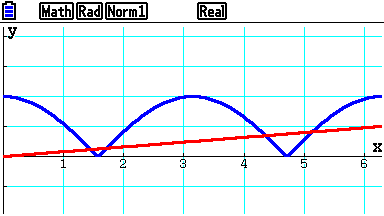
\includegraphics[width=0.4\textwidth]{./assets/5bi.png}
                              \end{center}

                        \item Hence, using the same axes, sketch a suitable straight line to determine the
                              number of solutions for the equation $4 \pi|\cos x|-x=0$ for $0 \leqslant x
                                  \leqslant 2 \pi$. State the number of solutions.

                              \sol{}
                              \begin{align*}
                                  4 \pi|\cos x| & = x              \\
                                  2|\cos x|     & = \frac{x}{2\pi}
                              \end{align*}
                              From the graph, the straight line intersects the curve at 4 points. Therefore, the number of solutions is 4.
                    \end{enumerate}
          \end{enumerate}

    \item Diagram 1 shows the sector $A O B$ of a circle with centre $O$ such that
          $\angle A O B$ is an acute angle. Given the perimeter and the area of the
          sector $A O B$ are $12 \mathrm{~cm}$ and $5 \mathrm{~cm}^2$ respectively.
          \begin{center}
              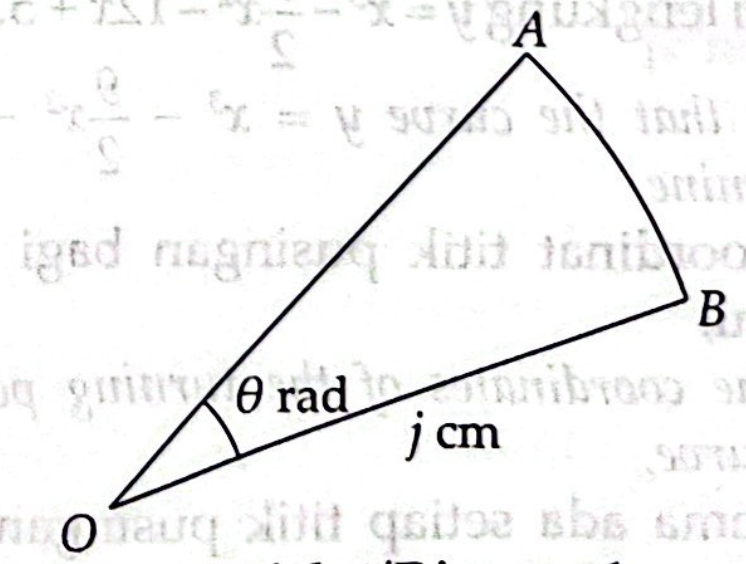
\includegraphics[width=0.3\textwidth]{./assets/6.png}
          \end{center}
          \begin{enumerate}
              \item Form two equations that relate $j$ and $\theta$ based on the above information.

                    \sol{}
                    \begin{align*}
                        \text{Perimeter} & = 2j + \theta j = 12\ \cdots\ (1) \\
                        \text{Area}      & = \frac{1}{2} \theta j^2 = 5      \\
                        \theta j^2       & = 10                              \\
                        \theta           & = \frac{10}{j^2}\ \cdots\ (2)
                    \end{align*}

                    \newpage
              \item Hence, find the value of $j$ and of $\theta$.

                    \sol{}
                    Substituting equation $(2)$ into equation $(1)$,
                    \begin{align*}
                        2j + \frac{10}{j^2} \cdot j & = 12                                \\
                        2j + \frac{10}{j}           & = 12                                \\
                        2j^2 + 10                   & = 12j                               \\
                        2j^2 - 12j + 10             & = 0                                 \\
                        j^2 - 6j + 5                & = 0                                 \\
                        (j-5)(j-1)                  & = 0                                 \\
                        j = 5\                      & \text{or}\ j = 1\ (\text{rejected}) \\
                        \theta                      & = \frac{10}{5^2} = \frac{10}{25}    \\
                                                    & = \frac{2}{5}                       \\
                                                    & = 0.4 \text{ rad}
                    \end{align*}
                    Therefore, $j=5$ and $\theta=0.4$ rad.
          \end{enumerate}

    \item \begin{enumerate}
              \item Determine the number of ways to form 4-digit odd numbers from the digits 4, 5,
                    7 and 9 if the number must be less than 7000.

                    \sol{}

                    First, choose the thousands place. Since the number must be less than 7000, the
                    thousands place can only be 4 or 5.

                    If the thousands place is 4, then the units place can be filled in 3 ways.

                    If the thousands place is 5, then the units place can be filled in 2 ways.

                    The tens and hundreds place can be filled in $\permtwo[2]{2} = 2$ ways.

                    The total number of ways to form the 4-digit odd numbers is $(3+2)2 = 10$.

              \item Diagram 2 shows a normal distribution graph which is symmetrical at $X=32$.

                    \begin{center}
                        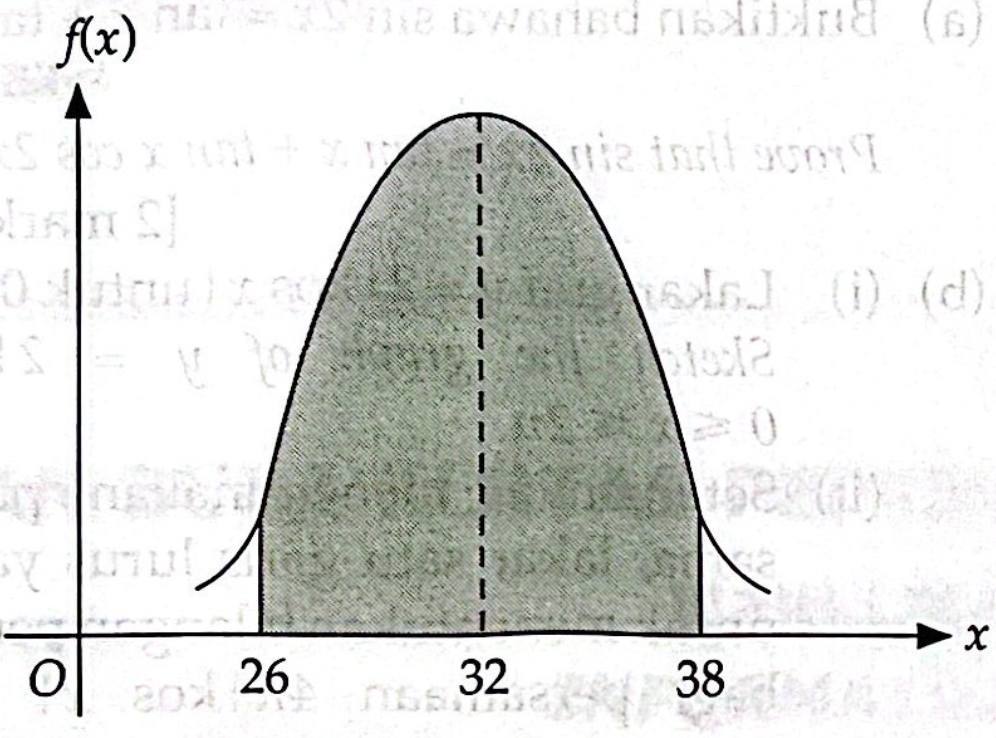
\includegraphics[width=0.4\textwidth]{./assets/7b.png}
                    \end{center}
                    \begin{enumerate}
                        \item State the mean, $\mu$.

                              \sol{}

                              The mean, $\mu = 32$.

                              \newpage

                        \item Express the shaded region in probability notation.

                              \sol{}

                              The shaded region is $P(26<X<38)$.

                        \item If the probability of the shaded region is 0.68 , find $P(X<26)$.

                              \sol{}
                              \begin{align*}
                                  P(X<26) & = 0.5 - \frac{0.68}{2} \\
                                          & = 0.5 - 0.34           \\
                                          & = 0.16
                              \end{align*}
                    \end{enumerate}
          \end{enumerate}

    \item \begin{enumerate}
              \item Find the equation of the tangent and normal to the curve $f(x)=x^3-3 x^2+6$ at
                    point $A(3,6)$.

                    \sol{}
                    \begin{align*}
                        f'(x) & = 3x^2 - 6x     \\
                        f'(3) & = 3(3)^2 - 6(3) \\
                              & = 27 - 18       \\
                              & = 9
                    \end{align*}
                    The gradient of the tangent is 9. The equation of the tangent is
                    \begin{align*}
                        y-6 & = 9(x-3)  \\
                        y   & = 9x-27+6 \\
                        y   & = 9x-21
                    \end{align*}
                    The gradient of the normal is $-\dfrac{1}{9}$. The equation of the normal is
                    \begin{align*}
                        y-6 & = -\frac{1}{9}(x-3)           \\
                        y   & = -\frac{1}{9}x+\frac{1}{3}+6 \\
                        y   & = -\frac{1}{9}x+\frac{19}{3}
                    \end{align*}

              \item Given that the curve $y=x^3-\dfrac{9}{2} x^2-12 x+5$. Determine
                    \begin{enumerate}
                        \item the coordinates of the turning point of the curve,

                              \sol{}
                              \begin{align*}
                                  y'           & = 3x^2 - 9x - 12 = 0   \\
                                  x^2 - 3x - 4 & = 0                    \\
                                  (x-4)(x+1)   & = 0                    \\
                                  x            & = 4\ \text{or}\ x = -1
                              \end{align*}
                              When $x=4$, $y=4^3-\dfrac{9}{2}(4)^2-12(4)+5=-51$. \\
                              When $x=-1$, $y=(-1)^3-\dfrac{9}{2}(-1)^2-12(-1)+5=\dfrac{23}{2}$. \\
                              The coordinates of the turning points are $(4,-51)$ and $\left(-1,\dfrac{23}{2}\right)$.

                        \item whether each turning point is a maximum or minimum point.

                              \sol{}
                              \begin{align*}
                                  y''(x)  & = 6x - 9          \\
                                  y''(4)  & = 6(4) - 9 = 15   \\
                                  y''(-1) & = 6(-1) - 9 = -15
                              \end{align*}
                              The turning point $(4,-51)$ is a minimum point and the turning point $\left(-1,\dfrac{23}{2}\right)$ is a maximum point.

                    \end{enumerate}
          \end{enumerate}
    \item Use graph paper to answer this question.

          Table 1 shows the values of two variables, $x$ and $y$, obtained from an
          experiment. The variables $x$ and $y$ are related by the equation $p y=x^2+q
              x$, where $p$ and $q$ are constants.

          \begin{center}
              \begin{tabular}{|c|c|c|c|c|c|c|}
                  \hline$x$ & 1 & 2 & 3 & 4  & 5  & 6  \\
                  \hline$y$ & 2 & 5 & 9 & 14 & 20 & 27 \\
                  \hline
              \end{tabular}
          \end{center}

          \begin{enumerate}
              \item Plot $\dfrac{y}{x}$ against $x$ by using a scale of $2 \mathrm{~cm}$ to 1 unit
                    on the $x$-axis and $2 \mathrm{~cm}$ to 0.5 unit on the $\dfrac{y}{x}$-axis.
                    Hence, draw the line of best fit.
              \item Using the graph in $9(a)$, find the value of
                    \begin{enumerate}
                        \item $p$,
                        \item $q$.
                    \end{enumerate}
          \end{enumerate}
          \sol{}

          Lazy to do this. =)

    \item Diagram 3 shows a straight line $A B$ which intersects a straight line $B C$ at
          point $B$. The point $C$ lies on the $y$-axis.
          \begin{center}
              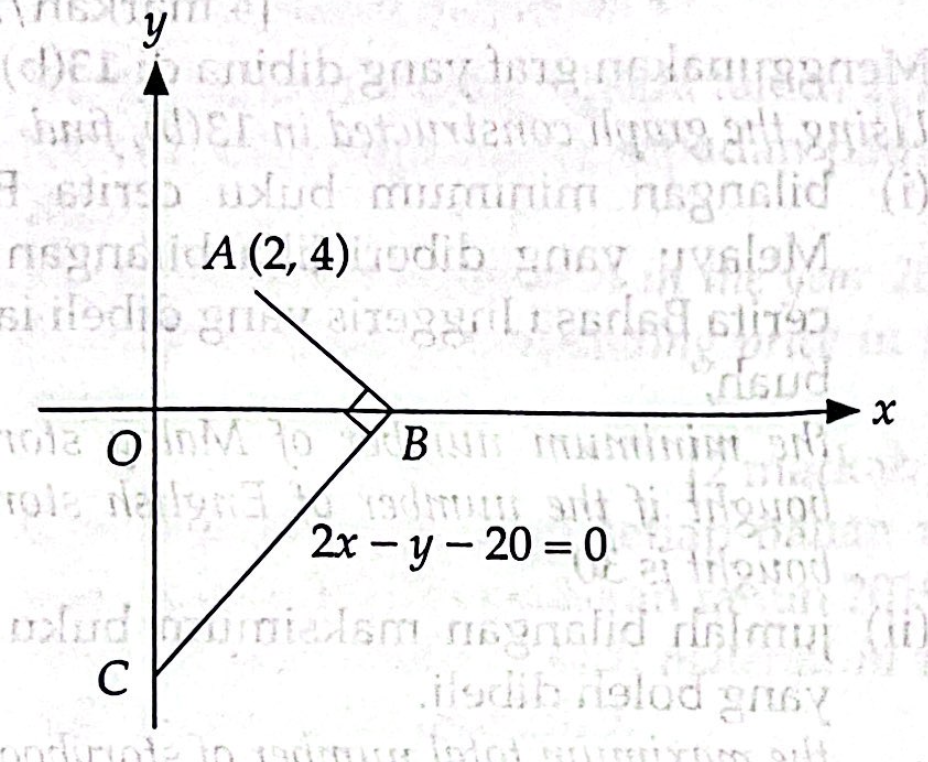
\includegraphics[width=0.4\textwidth]{./assets/10.png}
          \end{center}

          \newpage
          \begin{enumerate}
              \item Find
                    \begin{enumerate}
                        \item the equation of the straight line $A B$,

                              \sol{}
                              \begin{align*}
                                  2x - y -20 & = 0       \\
                                  y          & = 2x - 20 \\
                                  m          & = 2
                              \end{align*}
                              $\because$ $AB$ is perpendicular to the line $BC$.

                              $\therefore$ the gradient of $AB$ is $-\dfrac{1}{2}$.
                              \begin{align*}
                                  y - 4  & = -\frac{1}{2}(x-2) \\
                                  2y - 8 & = -x+2              \\
                                  x + 2y & = 10
                              \end{align*}

                        \item the coordinates of point $B$.

                              \sol{}

                              Point $B$ is touching the $x$-axis. Therefore, the $y$-coordinate of point $B$
                              is 0.

                              When $y=0$,
                              \begin{align*}
                                  0 & = 2x - 20 \\
                                  x & = 10
                              \end{align*}
                              Therefore, the coordinates of point $B$ are $(10,0)$.
                    \end{enumerate}

              \item The straight line $A B$ is extended to point $D$ such that $A B: B D=1: 3$.
                    Find the coordinates of point $D$.

                    \sol{}

                    Let the coordinates of point $D$ be $(x, y)$.
                    \begin{align*}
                        \left(\dfrac{3(2) + 1(x)}{4}, \dfrac{3(4) + 1(y)}{4}\right) & = (10,0) \\
                        \left(\dfrac{6 + x}{4}, \dfrac{12 + y}{4}\right)            & = (10,0) \\
                        \dfrac{6 + x}{4}                                            & = 10     \\
                        6 + x                                                       & = 40     \\
                        x                                                           & = 34     \\
                        \dfrac{12 + y}{4}                                           & = 0      \\
                        12 + y                                                      & = 0      \\
                        y                                                           & = -12
                    \end{align*}
                    Therefore, the coordinates of point $D$ are $(34,-12)$.

                    \newpage
              \item Point $P$ moves such that its distance from point $A$ is always 5 units. Find
                    the equation of the locus of point $P$.

                    \sol{}

                    The locus of point $P$ is a circle with centre $(2, 4)$ and radius 5.
                    \begin{align*}
                        (x-2)^2 + (y-4)^2            & = 5^2 \\
                        x^2 - 4x + 4 + y^2 - 8y + 16 & = 25  \\
                        x^2 + y^2 - 4x - 8y - 5      & = 0
                    \end{align*}

              \item Determine whether point $(2,6)$ lies in the locus of point $P$.

                    \sol{}
                    When $x=2$ and $y=6$,
                    \begin{align*}
                        2^2 + 6^2 - 4(2) - 8(6) - 5 & = 4 + 36 - 8 - 48 - 5 \\
                                                    & = -21 \neq 0
                    \end{align*}
                    Therefore, point $(2,6)$ does not lie in the locus of point $P$.
          \end{enumerate}
    \item \begin{enumerate}
              \item Find the range of values of $x$ if $(x-2)^2>16-3 x$.

                    \sol{}
                    \begin{align*}
                        (x-2)^2         & > 16-3x            \\
                        x^2-4x+4        & > 16-3x            \\
                        x^2-x-12        & > 0                \\
                        (x-4)(x+3)      & > 0                \\
                        x          < -3 & \ \text{or}\ x > 4
                    \end{align*}

              \item Diagram 4 shows the curve of a quadratic function $f(x)=x^2+m x+8$. The curve
                    has a minimum point $B(3, h)$ and intersects the $f(x)$-axis at point $A$.
                    \begin{center}
                        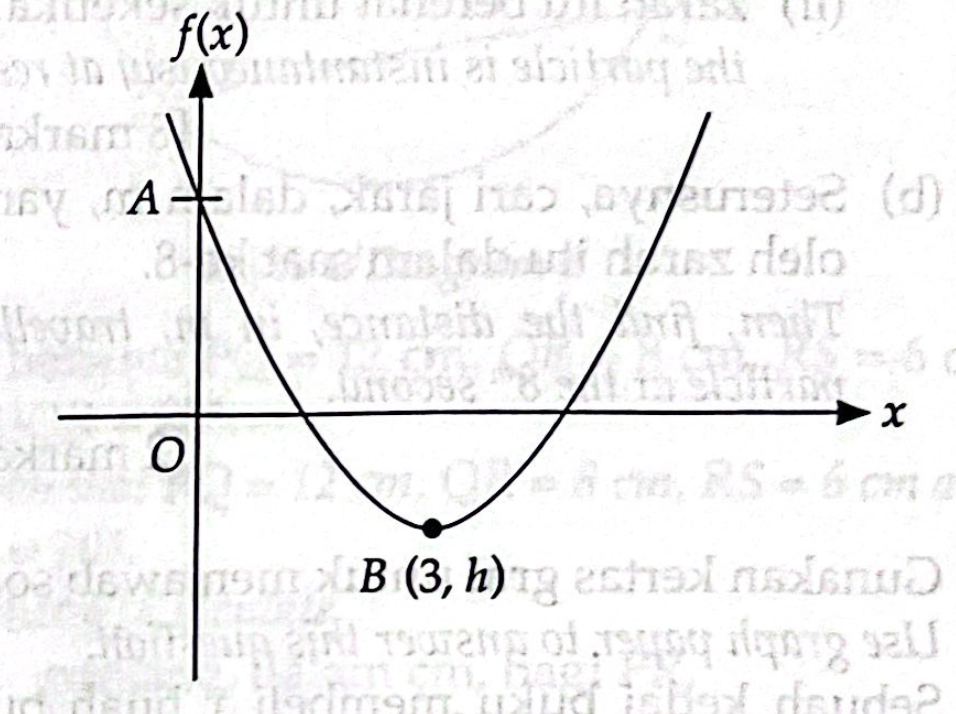
\includegraphics[width=0.4\textwidth]{./assets/11b.png}
                    \end{center}
                    \begin{enumerate}
                        \item Find the coordinates of point $A$.

                              \sol{}

                              When the curve intersects the $f(x)$-axis, $x=0$.
                              \begin{align*}
                                  f(0) & = 0^2 + m(0) + 8 \\
                                       & = 8
                              \end{align*}
                              Therefore, the coordinates of point $A$ are $(0,8)$.

                        \item By using the method of completing the square, find the value of $m$ and of $h$. 

                              \sol{}
                              \begin{align*}
                                  f(x) & = x^2 + m x + 8                                              \\
                                       & = \left(x^2 + m x + \frac{m^2}{4}\right) - \frac{m^2}{4} + 8 \\
                                       & = \left(x+\frac{m}{2}\right)^2 - \frac{m^2}{4} + 8           \\
                                       & = \left(x+\frac{m}{2}\right)^2 - \frac{m^2-32}{4}
                              \end{align*}
                              The minimum point is $\left(-\dfrac{m}{2}, \dfrac{m^2-32}{4}\right) = (3, h)$.
                              \begin{align*}
                                  -\frac{m}{2} & = 3  \\
                                  m            & = -6
                              \end{align*}
                              \begin{align*}
                                  h & = \frac{m^2-32}{4}    \\
                                    & = \frac{(-6)^2-32}{4} \\
                                    & = \frac{36-32}{4}     \\
                                    & = 1
                              \end{align*}
                              Therefore, $m=-6$ and $h=1$.

                        \item Determine the range of values of $x$ if $f(x)<8$.

                              \sol{}
                              \begin{align*}
                                  f(x)     & < 8   \\
                                  x^2-6x+8 & < 8   \\
                                  x^2-6x   & < 0   \\
                                  x(x-6)   & < 0   \\
                                  0 <      & x < 6
                              \end{align*}
                    \end{enumerate}
          \end{enumerate}

    \item A particle moves along a straight line and passes through a fixed point $O$
          with a velocity of $14 \mathrm{~m} \mathrm{~s}^{-1}$. Its acceleration, a
          $\mathrm{m} \mathrm{s}^{-2}$, at $t$ seconds after passing through $O$ is given
          by $a=5-2 t$.
          \begin{enumerate}
              \item Find the instantaneous displacement, in $m$, of the particle when
                    \begin{enumerate}
                        \item $t=3$

                              \sol{}
                              \begin{align*}
                                  a & = 5 - 2t            \\
                                  v & = \int a \, dt      \\
                                    & = \int (5-2t) \, dt \\
                                    & = 5t - t^2 + C
                              \end{align*}
                              When $t=0$, $v=14$.
                              \begin{align*}
                                  14 & = 5(0) - (0)^2 + C \\
                                  C  & = 14
                              \end{align*}
                              Therefore, $v=5t-t^2+14$.
                              \begin{align*}
                                  s & = \int v \, dt                              \\
                                    & = \int (5t-t^2+14) \, dt                    \\
                                    & = \frac{5}{2}t^2 - \frac{1}{3}t^3 + 14t + C
                              \end{align*}
                              When $t=0$, $s=0$.
                              \begin{align*}
                                  0 & = \frac{5}{2}(0)^2 - \frac{1}{3}(0)^3 + 14(0) + C \\
                                  C & = 0
                              \end{align*}
                              Therefore, $s=\dfrac{5}{2}t^2 - \dfrac{1}{3}t^3 + 14t$.
                              \begin{align*}
                                  s(3) & = \dfrac{5}{2}(3)^2 - \dfrac{1}{3}(3)^3 + 14(3) \\
                                       & = \dfrac{45}{2} - 9 + 42                        \\
                                       & = 55.5 \text{ m}
                              \end{align*}

                        \item the particle is insantaneously at rest.

                              \sol{}
                              \begin{align*}
                                  v          & = 0                                   \\
                                  5t-t^2+14  & = 0                                   \\
                                  t^2-5t-14  & = 0                                   \\
                                  (t-7)(t+2) & = 0                                   \\
                                  t= 7\      & \text{or}\ t = -2 \ (\text{rejected})
                              \end{align*}
                              When $t=7$,
                              \begin{align*}
                                  s & = \dfrac{5}{2}(7)^2 - \dfrac{1}{3}(7)^3 + 14(7) \\
                                    & \approx 106.17 \text{ m}
                              \end{align*}
                    \end{enumerate}

                    \newpage
              \item Then, find the distance, in $m$, travelled by the particle at the $8^{\text {th
                                }}$ second.

                    \sol{}
                    \begin{align*}
                        s & = \left|s(8) - s(7)\right|                                                                                                             \\
                          & = \left|\left(\dfrac{5}{2}(8)^2 - \dfrac{1}{3}(8)^3 + 14(8)\right) - \left(\dfrac{5}{2}(7)^2 - \dfrac{1}{3}(7)^3 + 14(7)\right)\right| \\
                          & = \left|-4\dfrac{5}{6}\right|                                                                                                          \\
                          & = 4\dfrac{5}{6} \text{ m}
                    \end{align*}
          \end{enumerate}

    \item Use graph paper to answer this question.

          A bookshop buys $x$ English storybooks and $y$ Malay storybooks. The prices of
          each English storybook and Malay storybook are RM40 and RM30 respectively. The
          purchase of the storybooks is based on the following constraints:

          \begin{enumerate}[label=\Roman{*}:]
              \item The total amount allocated is RM2 000.
              \item The number of Malay storybooks is not more than four times the number of
                    English storybooks.
              \item The number of English storybooks is at most three times the number of Malay
                    storybooks.
          \end{enumerate}
          \begin{enumerate}
              \item Write three inequalities, other than $x \geqslant 0$ and $y \geqslant 0$ that
                    satisfy all the given constraints.

                    \sol{}
                    \begin{enumerate}[label=\Roman{*}:]
                        \item $40x + 30y \leq 2000$
                        \item $y \leq 4x$
                        \item $x \leq 3y$
                    \end{enumerate}

              \item Using a scale of $2 \mathrm{~cm}$ to 10 storybooks on both axes, construct and
                    shade the region $R$ which satisfies all the given constraints.

                    \sol{}
                    \begin{center}
                        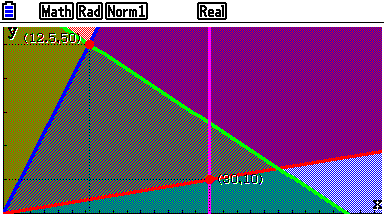
\includegraphics[width=0.4\textwidth]{./assets/13.4.png}
                    \end{center}
              \item Using the graph constructed in 13(b), find
                    \begin{enumerate}
                        \item the minimum number of Malay storybooks bought if the number of English
                              storybooks bought is 30,

                              \sol{}

                              According to the graph, the minimum number of Malay storybooks bought is 10.

                        \item the maximum total number of storybooks that can be bought.

                              \sol{}

                              According to the graph, the maximum total number of storybooks that can be
                              bought is 62.
                    \end{enumerate}
          \end{enumerate}
    \item Table 2 shows the price indices and changes in price indices of four raw
          materials, $A, B, C$ and $D$, used in the production of a type of snack in a
          factory.
          \begin{center}
              \begin{tabular}{|c|c|c|}
                  \hline \begin{tabular}{c}

                             Raw \\ material
                         \end{tabular} & \begin{tabular}{c}
                                             Price index in the \\
                                             year 2020 based    \\
                                             on the year 2019
                                         \end{tabular} & \begin{tabular}{c}
                                                             Change in price  \\
                                                             index from the   \\
                                                             year 2020 to the \\
                                                             year 2022
                                                         \end{tabular}              \\
                  \hline A                  & 130                                     & \begin{tabular}{c}

                                                                                            $15 \%$ increase
                                                                                        \end{tabular} \\
                  \hline$B$                 & 110                                     & \begin{tabular}{c}

                                                                                            $5 \%$ increase
                                                                                        \end{tabular} \\
                  \hline$C$                 & 150                                     & \begin{tabular}{c}

                                                                                            No change
                                                                                        \end{tabular} \\
                  \hline$D$                 & 140                                     & \begin{tabular}{c}

                                                                                            $10 \%$ decrease
                                                                                        \end{tabular} \\
                  \hline
              \end{tabular}
          \end{center}

          Diagram 5 shows a bar chart which represents the mass of the raw materials used
          to make the snacks in the year 2019.
          \begin{center}
              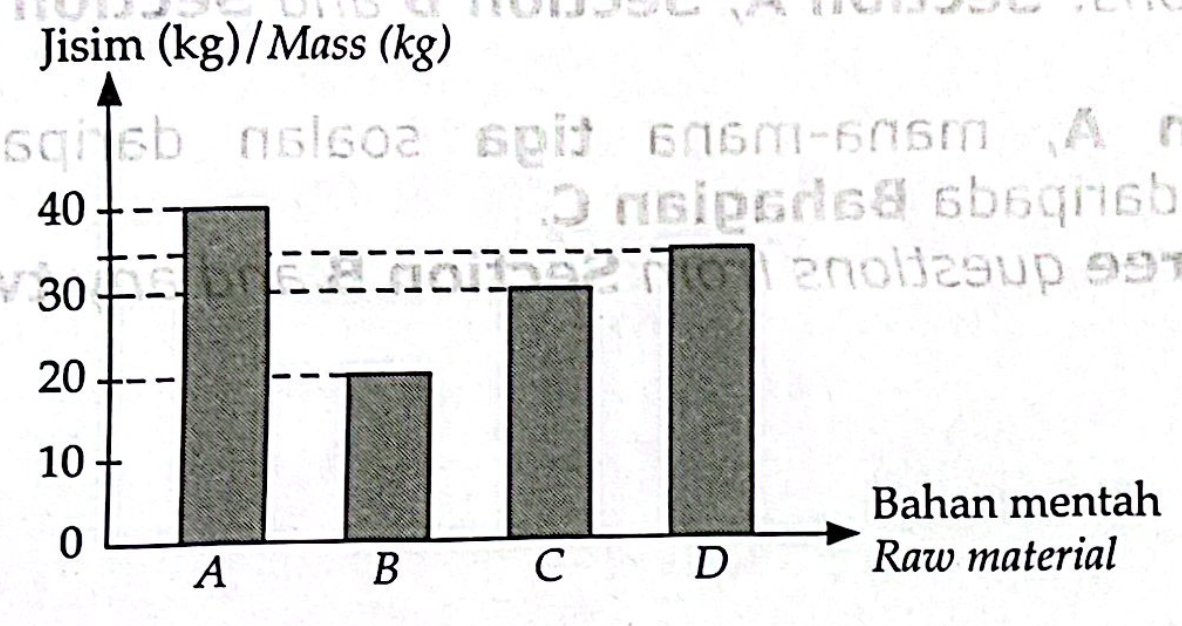
\includegraphics[width=0.5\textwidth]{./assets/14a.png}
          \end{center}
          \begin{enumerate}
              \item The price of raw material $A$ in the year 2020 was RM110. Find the
                    corresponding price in the year 2019.

                    \sol{}
                    \begin{align*}
                        \text{Price index} & = \frac{P_{2020}}{P_{2019}} \times 100 \\
                        130                & = \frac{110}{P_{2019}} \times 100      \\
                        P_{2019}           & = \frac{110}{130} \times 100           \\
                                           & = \text{RM }84.62
                    \end{align*}

              \item  Find the price index of each material in the year 2022 based on the year 2019.
                    \sol{}
                    \begin{align*}
                        \text{Price Index of A}_{2022/2019} & = 130 \times 115\% = 149.5 \\
                        \text{Price Index of B}_{2022/2019} & = 110 \times 105\% = 115.5 \\
                        \text{Price Index of C}_{2022/2019} & = 150 \times 100\% = 150   \\
                        \text{Price Index of D}_{2022/2019} & = 140 \times 90\% = 126
                    \end{align*}

                    \newpage
              \item \begin{enumerate}
                        \item Calculate the composite index for the cost of producing the snacks in the year
                              2022 based on the year 2019.

                              \sol{}
                              \begin{align*}
                                  \text{Composite index} & = \frac{149.5 \times 40 + 115.5 \times 20 + 150 \times 30 + 126 \times 35}{40+20+30+35} \\
                                                         & = \frac{5980 + 2310 + 4500 + 4410}{125}                                                 \\
                                                         & = \frac{17200}{125}                                                                     \\
                                                         & = 137.6
                              \end{align*}

                        \item Hence, find the cost of producing the snacks in the year 2019 if the
                              corresponding cost in the year 2022 is RM325.40.

                              \sol{}
                              \begin{align*}
                                  \dfrac{P_{2022}}{P_{2019}} \times 100 & = 137.6                            \\
                                  \dfrac{325.40}{P_{2019}} \times 100   & = 137.6                            \\
                                  P_{2019}                              & = \dfrac{325.40}{137.6} \times 100 \\
                                                                        & = \text{RM }236.48
                              \end{align*}
                    \end{enumerate}
          \end{enumerate}

    \item Diagram 6 shows a quadrilateral $P Q R S$ inscribed in a circle.

          It is given that $P Q=12 \mathrm{~cm}, Q R=8 \mathrm{~cm}, R S=6 \mathrm{~cm}$
          and $\angle P Q R=70^{\circ}$.
          \begin{center}
              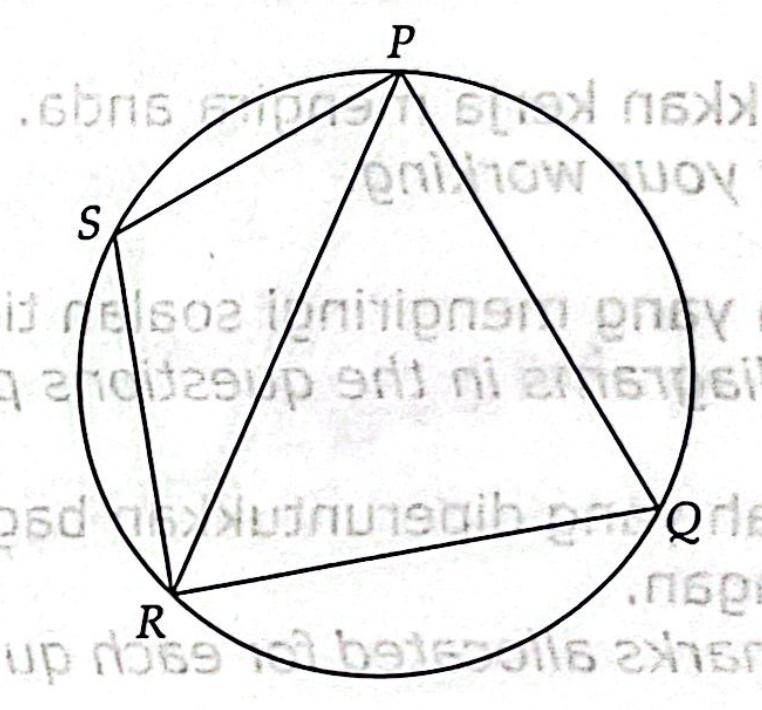
\includegraphics[width=0.4\textwidth]{./assets/1555.png}
          \end{center}
          \begin{enumerate}
              \item Calculate
                    \begin{enumerate}
                        \item the length, in $\mathrm{cm}$, of $P R$,

                              \sol{}
                              \begin{align*}
                                  PR & = \sqrt{12^2 + 8^2 - 2(12)(8)\cos 70^{\circ}} \\
                                     & \approx 11.93 \text{ cm}
                              \end{align*}

                        \item $\angle P R S$.

                              \sol{}
                              \begin{align*}
                                  \angle PSR                      & = 180^{\circ} - 70^{\circ}                  \\
                                                                  & = 110^{\circ}                               \\
                                  \dfrac{PR}{\sin \angle PSR}     & = \dfrac{RS}{\sin \angle SPR}               \\
                                  \dfrac{11.93}{\sin 110^{\circ}} & = \dfrac{6}{\sin \angle SPR}                \\
                                  \sin \angle SPR                 & = \dfrac{6 \sin 110^{\circ}}{11.93}         \\
                                                                  & \approx 0.47                                \\
                                  \angle SPR                      & \approx 28.20^{\circ}                       \\
                                  \angle PRS                      & = 180^{\circ} - 110^{\circ} - 28.20^{\circ} \\
                                                                  & = 41.80^{\circ}
                              \end{align*}
                    \end{enumerate}

              \item Find the area, in $\mathrm{cm}^2$, of triangle $P Q R$.

                    \sol{}
                    \begin{align*}
                        \text{Area of triangle } PQR & = \frac{1}{2} \times 12 \times 8 \times \sin 70^{\circ} \\
                                                     & \approx 45.11 \mathrm{~cm}^2
                    \end{align*}

              \item Find the shortest distance, in $\mathrm{cm}$, from point $Q$ to the straight
                    line PR.

                    \sol{}

                    The shortest distance from point $Q$ to the straight line $PR$ is the
                    perpendicular distance from point $Q$ to the straight line $PR$.

                    Let the shortest distance be $h$.
                    \begin{align*}
                        \dfrac{QR}{\sin \angle RPQ} & = \dfrac{PR}{\sin \angle PQR}      \\
                        \dfrac{8}{\sin RPQ}         & = \dfrac{11.93}{\sin 70^{\circ}}   \\
                        \sin RPQ                    & = \dfrac{8 \sin 70^{\circ}}{11.93} \\
                                                    & \approx 0.63                       \\
                        \angle RPQ                  & \approx 39.06^{\circ}              \\
                        \dfrac{h}{PQ}               & = \sin 39.06^{\circ}               \\
                        h                           & = 12 \sin 39.06^{\circ}            \\
                                                    & \approx 7.56 \mathrm{~cm}
                    \end{align*}
          \end{enumerate}
\end{enumerate}
\end{document}